\documentclass[a4paper,12pt]{article}
\usepackage[utf8]{inputenc}
\usepackage[ngerman]{babel}

\usepackage{amsmath}
\usepackage{amsthm}
\usepackage{amsfonts}
\usepackage{amssymb}
\usepackage[left=3cm,right=2cm,top=2cm,bottom=1.5cm]{geometry}
\usepackage{parskip}
\usepackage{graphicx}
\usepackage{caption}
\usepackage{hyperref}
\usepackage{upgreek}
\hypersetup{
    colorlinks,
    citecolor=black,
    filecolor=black,
    linkcolor=red,
    urlcolor=red
}

%%Code style
\usepackage{listings}
\usepackage{xcolor}
\definecolor{codegreen}{rgb}{0,0.6,0}
\definecolor{codegray}{rgb}{0.5,0.5,0.5}
\definecolor{codepurple}{rgb}{0.58,0,0.82}
\definecolor{backcolour}{rgb}{0.9,0.9,0.9}

\lstset{escapeinside={@}{@}}
\lstdefinestyle{mystyle}{
    backgroundcolor=\color{backcolour},   
    commentstyle=\color{codegreen},
    keywordstyle=\color{magenta},
    numberstyle=\tiny\color{codegray},
    stringstyle=\color{codepurple},
    basicstyle=\ttfamily\footnotesize,
    breakatwhitespace=false,         
    breaklines=true,                 
    captionpos=b,                    
    keepspaces=true,                 
    numbers=left,                    
    numbersep=5pt,                  
    showspaces=false,                
    showstringspaces=false,
    showtabs=false,                  
    tabsize=5
}

\lstset{style=mystyle}

\newcommand{\blue}[1]{\textcolor{blue}{#1}}
\newcommand{\orange}[1]{\textcolor{orange}{#1}}
%%End code style

\title{Computer System Sicherheit\\Notizen WS20/21}
\author{Felix Marx}

\begin{document}
\maketitle

{
%%Lokales Einfärben des Inhaltverzeichisses
\hypersetup{linkcolor=black}
\tableofcontents
}
\newpage

\section{Begriffe}
Unterscheidung \blue{Betriebssicherheit (safety)} und \blue{Angriffssicherheit (security)}.\\
safety bezeichnet den Schutz vor inneren Fehlern, deren Eintrittswahrscheinlichkeit durch probabilistische Techniken ermittelt wird.\\
security den Schutz gegen aktive Angreifer.

\subsection{Security}

Trends und Herausforderungen:\\
\textbf{Mobilität}, der Übergang zu ''smart devices''
\begin{figure}[h!]
\centering
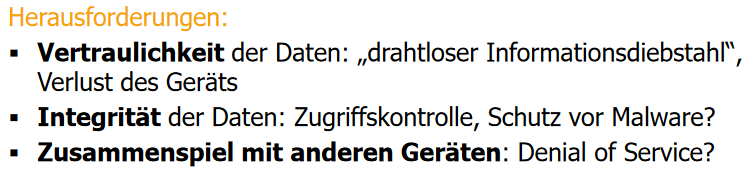
\includegraphics[scale=0.6]{Grafiken/Trend-Mobilitaet.png}
\caption{Herausforderungen bei der Mobilität}
\end{figure}

\textbf{Vernetzung}, der Übergang zu ''always on'' und Automatisierung von Systemen
\begin{figure}[h!]
\centering
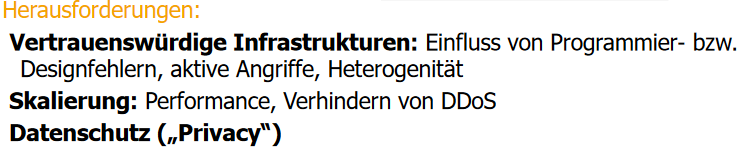
\includegraphics[scale=0.6]{Grafiken/Trend-Vernetzung.png}
\caption{Herausforderungen bei der Vernetzung}
\end{figure}

\textbf{Miniaturisierung}, Produktion kleinerer Chips mit Trend zu Einwegchips
\begin{figure}[h!]
\centering

\includegraphics[scale=0.6]{Grafiken/Trend-Miniaturisierung.png}
\caption{Herausforderungen bei der Mobilität}
\end{figure}\\

\blue{Social Engineering} bezeichnet das Erlangen von vertraulichen Daten durch psychologische Techniken\\
\blue{Man-in-the-middle} Angriffe, hier werden Nachrichten vor der gesicherten Kommunikation abgefangen.\\
Lösungen für \blue{Phishing} umfassen die Verifikation durch Transaktionsnummern (TANs) oder Hardwaretokens was allerding nicht die Integrität der Transaktion gewährleistet.\\
Schutzmechanismen:\\
\blue{Passive Authentication}: Sicherstellung der Authentizität durch Einsatz einer digitalen Signatur\\
\blue{Basic Access Control}: elektronische gespeicherte Daten werden erst übermittelt wenn das Lesegerät einen aufgedruckten maschinenlesbaren Code kennt.\\
\blue{Active Access Control}: Verhindert 1:1 Kopien indem ein geheimer Schlüssel in einem gesicherten Chip-Bereich gespeichert wird.\\
\blue{Extended Access Control}: Schutz von sensiblen Daten (Fingerabdruck, Iris, etc.) durch das Abgleichen von \href{https://en.wikipedia.org/wiki/Extended_Access_Control}{Zertifikaten} die nur eine kurze Zeit gültig sind.

\subsection{Safety}
Im Fehlerfall sollte ein System immer in den sicheren Zustand übergehen.\\
Zum Beispiel zeigt die Fahranweisung von Zügen nach oben, sodass es bei einem Schaden am Mechanismus in den Haltezustand nach unten fällt (Schwerkraft). Ein Watchdog (hier Schwerkraft) überwacht quasi das System auf Fehler und resettet es bei einem Fehler.

\section{Verlässliche Systeme}
Ein zuverlässiges System erfüllt seinen Zweck auch falls Fehler auftreten.
\begin{figure}
\centering
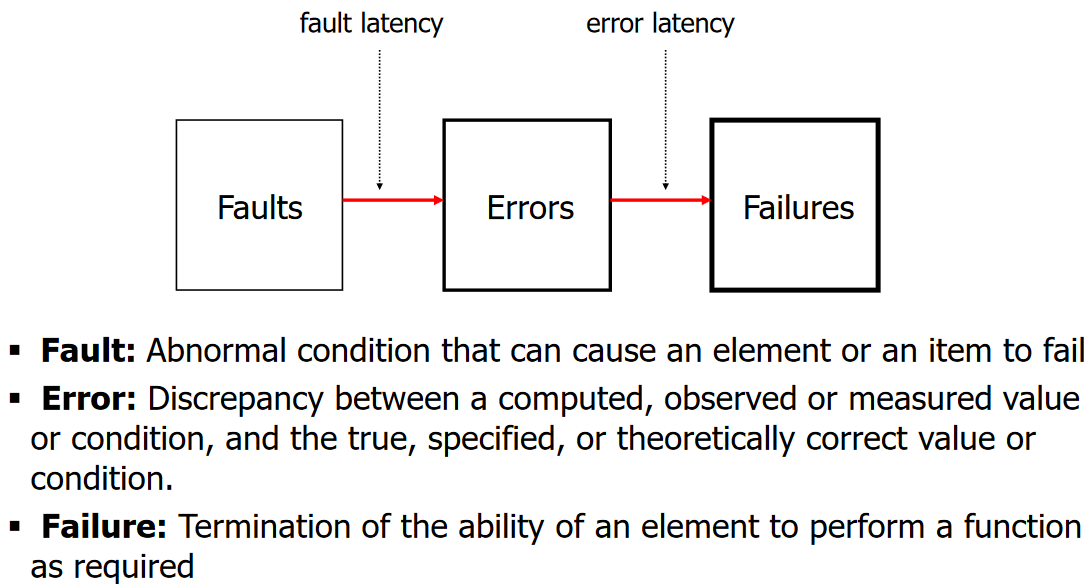
\includegraphics[scale=0.4]{Grafiken/AblaufZumVersagen.png}
\caption{Ablauf bis ein System versagt}
\label{Image:Versagensplan}
\end{figure}
Als Beispiel des \hyperref[Image:Versagensplan]{Ablaufes} lässt sich die Einwirkung von kosmischer Strahlung auf eine DRAM-Zelle (Fault) was zum Wechsel eines Wertes führt (Error), wodurch die Berechnung ein falsches Ergebnis liefert (Failure).\\
In der Zuverlässigkeit wird unterschieden nach:\\
\textbf{Availability}: Verfügbarkeit eines Systems gemessen in Prozent, d.h. 
$$\frac{\textrm{Total Up Time}}{\textrm{Total (Up + Down Time)}}=\frac{\textrm{MTTF}}{\textrm{MTTF + MTTR}}$$
\textbf{Reliability}: Zuverlässigkeit eines Systems, d.h. die Wahrscheinlichkeit dass ein System über einen gewissen Zeitraum korrekt funktioniert.\\
Wir bezeichnen mit \blue{MTTF} die Mean Time To Failure und mit \blue{MTTR} Mean Time To Recovery. Bei der Berechnung wird für die Up/Downtime nur die Zeiten im vereinbarten Betriebszeitraum gezählt!\\
Die Wahrscheinlichkeit, dass ein System bis zum Zeitpunkt $t$ fehlerhaft wird lässt sich mittels einer Verteilerfunktion $F$ und der Lebenszeit des Systems T berechnen:
$$F(t)=P(T\leq t)\textrm{, } R(t)=P(T>t)=1-F(t)$$
Die Funktion $R$ hingegen ermittelt die Wahrscheinlichkeit, dass ein System bis zum Zeitpunkt $t$ korrekt funktioniert.
Geht man davon aus, dass zukünftige Ausfälle unabhängig davon passieren, wann der letzte Ausfall war, lässt sich die Wahrscheinlichkeit mit einer Fehlerrate $\lambda$ so ausdrücken:\\
\begin{align*}
f(x) = &
\begin{cases} 
	\lambda e^{-\lambda x} & x\geq 0\\
	 0 & x < 0
\end{cases} \\
F(t) = & \int_{-\infty}^t f(x)dx = &
\begin{cases}
1 -e^{-\lambda t} & t \geq 0\\
0 & t < 0
\end{cases}\\
R(t) = & 1 -F(t) = & 
\begin{cases}
e^{-\lambda t} & t \geq 0\\
1 & t< 0
\end{cases}
\end{align*}
\begin{figure}[h!]
\centering
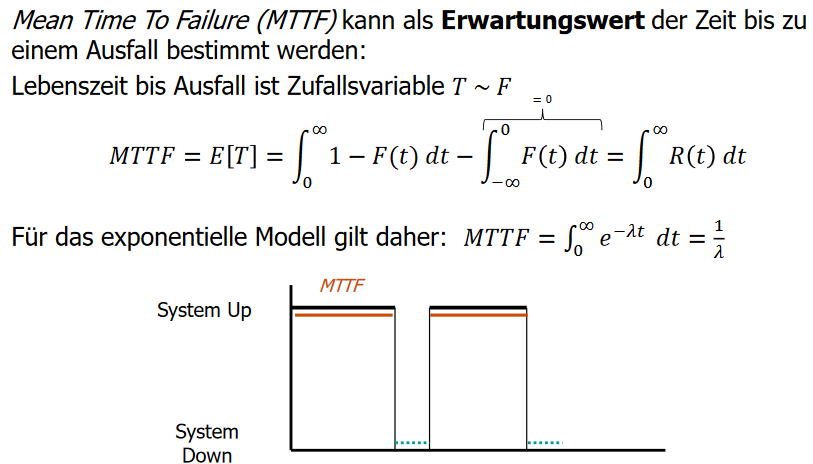
\includegraphics[scale=0.6]{Grafiken/MTTF-Model.png}
\caption{Berechnung MTTF mit dem exponentiellen Model}
\end{figure}\\
Bei in Reihe geschalteten Komponenten wird die Wahrscheinlichkeit dass das gesamte System korrekt funktioniert R durch $R_{ges}(t)=\prod^n_{i=1}R_i(t)$ im exponentiellen Modell wird dann für $\lambda = \lambda_{ges}=\sum_{i=1}^n\lambda_i$ verwendet.\\
Bei Parallelschaltung ist die Wahrscheinlichkeit dass das System korrekt funktioniert:
$$R_{ges}(t)=R_1(t)+R_2(t)-R_1(t)\cdot R_2(t), F_{ges}(t)=F_1(t)\cdot F_2(t)$$
Bei mehr als zwei Komponenten ist die allgemeine Formel:
$$R_{ges}(t)=1-\prod_{i=1}^n(1-R_i(t)), F_{ges}(t)=\prod_{i=1}^nF_i(t)$$

\subsection{Strategien zur Fehlervermeidung/toleranz}
\begin{itemize}
\item Fehlervermeidung (fault avoidance)
	\begin{itemize}
	\item Design des Systems stellt sicher, dass Fehler nicht auftreten
	\item Beispiel: Testen, Verifikation,...
	\end{itemize}
\item Wiederherstellung aus Fehlerzustand (fault recovery)
	\begin{itemize}
	\item Strategien, um ein System beim Auftreten eines Fehlers wieder in einen korrekten Systemzustand zu bringen
	\end{itemize}
\item Fehlertoleranz (fault tolerance)
	\begin{itemize}
	\item Wenn Fehler nicht vermieden werden können, dann soll das System Fehler tolerieren
	\item Beispiele: Redundanz, Safety, ...
	\end{itemize}
\end{itemize}
\textbf{Arten von Redundanzen:}
\begin{itemize}
\item Physikalische Redundanz (physical redundancy)
	\begin{itemize}
	\item Zusätzliche Ressourcen bzw. Komponenten
	\item Berechnungen werden auf mehreren Komponenten ausgeführt und verglichen
	\item Statische Redundanz
		\begin{itemize}
		\item $N$ Systeme laufen parallel
		\item $N-1$ Systeme laufen im  ''stand-by-mode''
		\item Bei einem Fehler wird im Betrieb umgeschaltet
		\item Dazu muss man den Fehler natürlich zuerst erkennen!
		\end{itemize}
	\item Dynamische Redundanz
		\begin{itemize}
		\item $N$ Systeme laufen parallel
		\item Ausfallsicherhere Komponente vergleicht die Resultate
		\item Mehrheitsentscheidung (zB. 2-out-of-3)
		\item Erkennt Fehler ''automatisch''
		\end{itemize}
	\end{itemize}
\item Zeitliche Redundanz (temporal redundancy)
	\begin{itemize}
	\item Berechnungen auf gleicher Hardware-Plattform wiederholen
	\end{itemize}
\item Redundanzen durch (Zusatz-)Information (information redundancy)
	\begin{itemize}
	\item Hinzufügen von zusätzlichen Daten (Checksummen, ...)
	\item Erlaubt Datenfelder bei Übertragung oder Speicherung zu erkennen
	\end{itemize}
\end{itemize}
Bei dynamischer Redundanz wird das Ergebnis parallel berechnet und dann per Mehrheitsentscheidung das korrekte ausgewählt. Problematisch falls im Vergleich ein Problem auftritt. Softwarefehler sind von der Hardware-Redundanz nicht abgedeckt.
Zusatzinformationen können die Integrität gesendeter Daten durch Checksummen sicherstellen, allerdings auch nur begrenzt.\\

Nachteile von Redundanzen sind:
\begin{itemize}
\item Schlechtere Performanz (bei temporaler Redundanz)
\item Synchronisation erforderlich
\item Hohe Kosten durch mehrfache Hardware bzw. mehrfache Implemenation (falls überhaupt möglich)
\item Benötigt Mechanismen zur Fehler-Erkennung, welche selbst wieder Fehleranfällig sein können
\end{itemize}

\section{Krypographie}
\begin{itemize}
\item Vertraulichkeit (Confidentiality)
	\begin{itemize}
	\item Schutz vor unbefugten Zugriff auf Informationen / Daten
	\end{itemize}
\item Integrität
	\begin{itemize}
	\item Schutz vor Veränderung von Informationen / Daten
	\end{itemize}
\item Verfügbarkeit (Availability)
	\begin{itemize}
	\item Daten oder Systeme sind verfügbar oder erreichbar
	\end{itemize}
\item Autehntizität (Authenticity)
	\begin{itemize}
	\item Schutz vor Fälschung von Informationen / Daten
	\end{itemize}
\item Nicht-Abstreitbarkeit (Non-Repudiation)
	\begin{itemize}
	\item Aktion ist nachprüfbar und kann nicht abgestritten werden
	\end{itemize}
\end{itemize}
\subsection{Begriffe}
\begin{itemize}
\item Klartext/Nachricht: eine zu verschlüsselnde Information
\item Klartextraum: Menge aller möglichen Klartexte
\item Chiffrat, Chiffretext: Verschlüsselte Nachricht
\item Chiffretextraum: Menge aller möglichen Chiffrate
\item Schlüssel: Ein Geheimnis, welches zur Ent-/Verschlüsselung benötigt wird
\item Schlüsselraum: Menge aller möglichen Schlüssel
\item Verschlüsselung: Umwandlung eines Klartext in ein Chiffrat
\item Entschlüsselung: Umwandlung eines Chiffrats in einen Klartext
\end{itemize}
\textbf{Kerckhoffs Prinzipien}
\begin{enumerate}
\item Das System muss praktisch, wenn nicht sogar mathematisch, unentschlüsselbar sein (''Unentschlüsselbarkeit'')
\item Es darf keine Geheimhaltung erfordern und darf ohne Schwierigkeiten  in die Hände des Feindes fallen (''Keine Geheimhaltung des Systems'')
\item Der Schlüssel muss ohne Hilfe geschriebener Notizen kommunizierbar und aufbewahrbar sein und er muss ausgewechselt oder modifiziert werden können nach Belieben der Kommunikationspartner (''Schlüssel ohne Aufschreiben'')
\item Es muss anwendbar sein auf die telegraphische Kommunikation
\item Es soll protabel sein und seine Funktion soll nicht die Zusammenkunft mehrerer Personen erfordern 
\item Schließlich ist es notwendig, angesichts der Umstände, unter denen es angewendet werden soll, dass das System einfach benutzbar ist und weder große gedankliche Anstrengung erfordert noch die Kenntnis einer langen Liste zu beachtender Regeln (''einfach benutzbar'')
\end{enumerate}
\subsection{Verschiebechiffre}
Die Ceasar-Chiffre ersetzt jeden Buchstaben des Klartextes durch den Buchstaben 3 Stellen weiter rechts, beim Entschlüsseln genau umgekehrt.\\
Die Verschiebechiffre ersetzt alle Buchstaben durch den Buchstaben welcher eine beliebige aber feste Anzahl an Stellen weiter rechts steht. Der Schlüssel ist die Anzahl an Verschiebungen, d.h. 0,1,2,...,25.

\subsection{Mathematische Grundlagen}
Als \blue{Einwegfunktionen} bezeichnet man Funktionen bei denen es ''einfach'' ist den Funktionswert $y = f(x)\in Y$ zu bestimmen, aber ''schwer'' ein Urbild $x\in f^{-1}[\{y\}]$ zu finden. Die Existenz von Einwegfunktionen ist nicht bewiesen (P/NP).
\subsubsection{Teilbarkeitsregeln}
\begin{align}
a | a\\
a | b \wedge b |c \Rightarrow a|c\\
a|b\wedge b\neq 0 \Rightarrow |a|\leq |b|\\
a | b\wedge b|a \Rightarrow |a| = |b|
\end{align}
Sind $a,n\in\mathbb{Z}$ mit $n\neq 0$, dann gibt es eindeutig bestimmte Zahlen $q,r\in\mathbb{Z}$ sodass
\begin{align*}
a= qn+r\\
0\leq r < |n|\\
q = \lfloor \frac{a}{n} \rfloor \wedge r = a -qn
\end{align*}
\subsubsection{Größter gemeinsamer Teiler}
\begin{align}
\textrm{ggT}(a,0)=|a|\\
\textrm{ggT}(a,1)=1\\
\textrm{ggT}(a,b)=\textrm{ggT}(b,a)\\
\textrm{ggT}(a,b)=\textrm{ggT}(|a|,|b|)\\
\textrm{ggT}(a,b)=\textrm{ggT}(b,a-b)\\
\textrm{Für } b\neq 0 \textrm{ gilt } \textrm{ggT}(a,b)=\textrm{ggT}(b,a \textrm{ mod } b)
\end{align}

Lineare diophantische Gleichung: $ax+by=c$\\
Eine diophantische Gleichung kann wie folgt gelöst werden.\\
Löse $ax'+by'=$ggT(a,b) und definiere $x=\frac{c}{\textrm{ggT(a,b)}}\cdot x'$, $y=\frac{c}{\textrm{ggT(a,b)}}\cdot y'$

\textbf{Beispiel erweiteter Euklid:}
$1337\cdot x+42\cdot y=\blue{7}$\\
\begin{tabular}{|l|l|l|l|l|}
a & b & $\lfloor \frac{a}{b} \rfloor$ & x & y\\
\hline
1337 & 42 & 31 & -1 & $1-31*(-1)=32$\\
\hline
42 & 35 & 1 & 1 & $0-1*1=-1$\\
\hline
35 & 7 & 5 & 0 & 1\\
\hline
\blue{7} & 0 & & 1 & 0
\end{tabular}\\
\subsubsection{Primzahlen}
Fundamentalsatz der Arithmetik:\\
Jede natürliche Zahl $n>1$ besitzt eine Zerlegung in ein Produkt aus Primzahlen, welche bis auf die Reihenfolge eindeutig ist.\\
Es gibt unendlich viele Primzahlen.\\

Die Eulersche-Phi-Funktion $$\varphi (b)=|\{a\in\mathbb{N} : a < b, \textrm{ggT}(a,b)=1\}|$$ beschreibt dei Anzahl der zu b teilerfremden Zahlen.\\
Für eine Primzahl p gilt $\varphi (p)=p-1$ und $\varphi (p^n)=p^n-p^{n-1}$.\\
Für teilerfremde Zahlen $a,b\in \mathbb{N}$ gilt $\varphi (ab)=\varphi (a)\cdot \varphi (b)$.\\
Sind $m,n\in \mathbb{N}$ teilerfremd, dann gilt $m^{\varphi (n)}\textrm{mod }n= 1$.\\
\textbf{Kleiner Satz von Fermat:}\\
Für eine Primzahl p und ein teilerfremde Zahl $m\in \mathbb{N}$ gilt $m^{p-1} \textrm{mod }p = 1$.

\end{document}